\documentclass[12pt]{article}
\usepackage{fullpage}
\usepackage{titlesec}
\usepackage{tikz}
\usepackage{amsfonts,amssymb}
\usepackage{amsmath}
\usepackage{comment}
\usetikzlibrary{automata, positioning}

\input ../libraries/mac.tex
\input ../libraries/mathmac.tex

\begin{document}
\pagestyle{plain}
\titleformat{\subsection}[runin]
  {\normalfont\large\bfseries}{\thesubsection}{1em}{}
\titleformat{\subsubsection}[runin]
  {\bfseries}{}{1em}{}

\title{Homework 6}
\author{Brooke Fugate, Michael O'Connor, Rohan Shah}
\date{}

\maketitle

\newpage
\section*{Problem B1}
\subsection*{(i)}
NFA $N_{C_G}$ for the grammer $G$:
\begin{center}
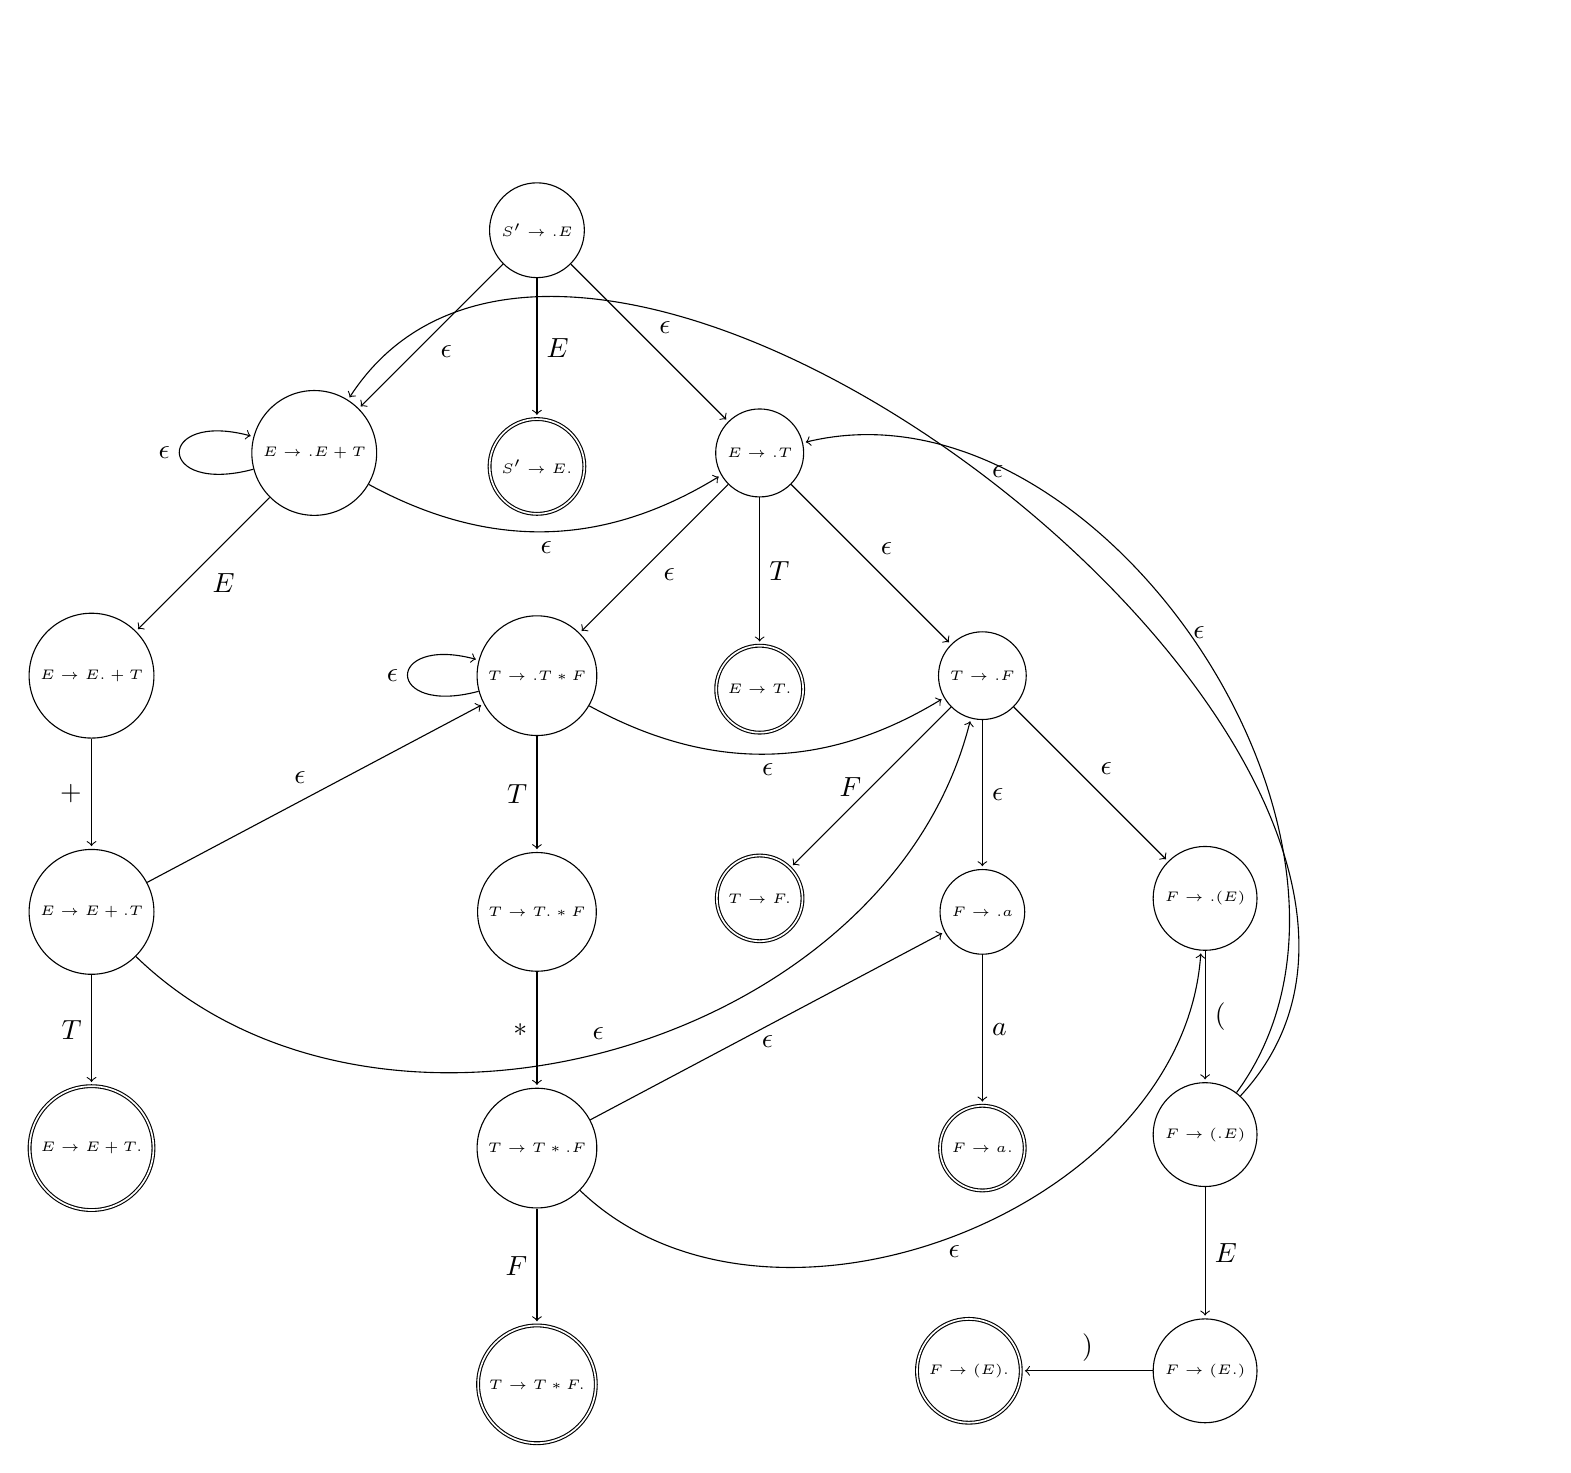
\begin{tikzpicture}[shorten >=1pt, node distance=3cm, on grid, auto]
  \node[state] (q0) {\tiny $S' \rightarrow .E$};
  \node[state, accepting] (q1) [below=of q0] {\tiny $S' \rightarrow E.$};
  \begin{scope}[node distance=4cm]
  \node[state] (q2) [below left=of q0] {\tiny $E \rightarrow .E+T$};
  \node[state] (q3) [below right=of q0] {\tiny $E \rightarrow .T$};
  \node[state] (q4) [below left=of q2] {\tiny $E \rightarrow E.+T$};
  \end{scope}
  \node[state, accepting] (q5) [below=of q3] {\tiny $E \rightarrow T.$};
  \begin{scope}[node distance=4cm]
  \node[state] (q6) [below left=of q3] {\tiny $T \rightarrow .T*F$};
  \node[state] (q7) [below right=of q3] {\tiny $T \rightarrow .F$};
  \end{scope}
  \node[state] (q8) [below=of q4] {\tiny $E \rightarrow E+.T$};
  \node[state] (q9) [below=of q6] {\tiny $T \rightarrow T.*F$};
  \node[state] (q12) [below=of q7] {\tiny $F \rightarrow .a$};
  \begin{scope}[node distance=4cm]
  \node[state, accepting] (q10) [below left=of q7] {\tiny $T \rightarrow F.$};
  \node[state] (q11) [below right=of q7] {\tiny $F \rightarrow .(E)$};
  \end{scope}
  \node[state, accepting] (q13) [below=of q8] {\tiny $E \rightarrow E+T.$};
  \node[state] (q14) [below=of q9] {\tiny $T \rightarrow T*.F$};
  \node[state] (q15) [below=of q11] {\tiny $F \rightarrow (.E)$};
  \node[state, accepting] (q16) [below=of q12] {\tiny $F \rightarrow a.$};
  \node[state, accepting] (q17) [below=of q14] {\tiny $T \rightarrow T*F.$};
  \node[state] (q18) [below=of q15] {\tiny $F \rightarrow (E.)$};
  \node[state, accepting] (q19) [left=of q18] {\tiny $F \rightarrow (E).$};

  \path[->]
  (q0) edge node {$E$} (q1)
  (q0) edge node {$\epsilon$} (q2)
  (q0) edge node {$\epsilon$} (q3)
  (q2) edge node {$E$} (q4)
  (q2) edge [loop left] node {$\epsilon$} (q2)
  (q2) edge [bend right] node [below] {$\epsilon$} (q3)
  (q3) edge node {$T$} (q5)
  (q3) edge node {$\epsilon$} (q6)
  (q3) edge node {$\epsilon$} (q7)
  (q4) edge node [left] {$+$} (q8)
  (q6) edge node [left] {$T$} (q9)
  (q6) edge [loop left] node {$\epsilon$} (q6)
  (q6) edge [bend right] node [below] {$\epsilon$} (q7)
  (q7) edge node [left] {$F$} (q10)
  (q7) edge node {$\epsilon$} (q11)
  (q7) edge node {$\epsilon$} (q12)
  (q8) edge node [left] {$T$} (q13)
  (q8) edge node {$\epsilon$} (q6)
  (q8) edge [bend right=60] node {$\epsilon$} (q7)
  (q9) edge node [left] {$*$} (q14)
  (q11) edge node {$($} (q15)
  (q12) edge node {$a$} (q16)
  (q14) edge node [left] {$F$} (q17)
  (q14) edge [bend right=65] node [below] {$\epsilon$} (q11)
  (q14) edge node [below] {$\epsilon$} (q12)
  (q15) edge node {$E$} (q18)
  (q15) edge [bend right=95] node [above] {$\epsilon$} (q2)
  (q15) edge [bend right=70] node [above] {$\epsilon$} (q3)
  (q18) edge node [above] {$)$} (q19)
  ;
\end{tikzpicture}
\end{center}

\newpage
\subsection*{(ii)}
DFA $D_{C_G}$ for the grammer $G$:
\newline
\begin{tikzpicture}[shorten >=1pt, node distance=3cm, on grid, auto]
  \node[state] (0) {0};
  \node[state] (4) [below=of 0] {4};
  \begin{scope}[node distance=2cm]
  \node[state, accepting] (3) [left=of 4] {3};
  \node[state, accepting] (1) [left=of 3] {1};
  \end{scope}
  \node[state, accepting] (5) [right=of 0] {5};
  \node[state] (6) [below=of 1] {6};
  \node[state] (8) [below=of 4] {8};
  \node[state, accepting] (2) [right=of 8] {2};
  \node[state] (7) [below=of 2] {7};
  \node[state, accepting] [below=of 6] (9) {9};
  \node[state, accepting] [right=of 7] (10) {10};
  \begin{scope}[node distance=2.5cm]
  \node[state, accepting] [below=of 8] (11) {11};
  \end{scope}

  \path[->]
  (0) edge node [above] {E} (1)
  (0) edge [bend left] node {T} (2)
  (0) edge node [left] {F} (3)
  (0) edge node [left] {(} (4)
  (0) edge node {a} (5)
  (1) edge node [left] {+} (6)
  (2) edge node {*} (7)
  (4) edge node [left] {E} (8)
  (4) edge node {T} (2)
  (4) edge node [above] {F} (3)
  (4) edge [loop right] node {(} (4)
  (4) edge node [below] {a} (5)
  (6) edge node [left] {T} (9)
  (6) edge node [above] {F} (3)
  (6) edge node [below] {(} (4)
  (6) edge [bend left=100] node {a} (5)
  (7) edge node {F} (10)
  (7) edge node {(} (4)
  (7) edge [bend right] node [right] {a} (5)
  (8) edge node [left] {)} (11)
  (8) edge node {+} (6)
  (9) edge [bend right] node [below] {*} (7)
  ;
\end{tikzpicture}

\newpage
\subsection*{(iii)} Let $G$ be a reduced context-free grammar where
$G = (V,\Sigma,P,S')$ and let $C_G$ be the set of characteristic strings of $G$
defined as:
$$C_G = \{\alpha\beta \in V^* \mid S' \underset{rm}{\Longrightarrow}^* \alpha Bv
\underset{rm}{\Longrightarrow} \alpha\beta v,\ \alpha,\beta \in V^*,\ v\in
\Sigma^*,\ B \rightarrow \beta \in P \}$$
Let $N_{C_G} = (Q,\Sigma,\delta,q_0,F)$ be the NFA constructed according to the
method described in Section 1 of the handout
\textit{A Survey of LR-Parsing Methods etc.}
\medskip\newline
\textbf{Claim:} For every rightmost derivation
$$A \overset{n}{\underset{rm}{\Longrightarrow}} \alpha Bv
\underset{rm}{\Longrightarrow}
\alpha\beta v \text{ implies } \delta^*((A \rightarrow \text{ "."}\zeta)
,\ \alpha\beta) = (B \rightarrow \beta\text{"."})$$
where $n\ge 0,\ v \in \Sigma^*$, $A,B\in N$, $\alpha,\beta\in V^*$,
$(A \rightarrow \text{ "."}\zeta)\in Q$, $(B \rightarrow \beta\text{"."})\in F$
and $A \rightarrow \zeta$ is the first production in the above rightmost
derivation.
\medskip\newline
\textbf{Proof:} By induction on the n.
\medskip\newline
\textbf{Base Case:} n = 0. So we have
$$A \underset{rm}{\Longrightarrow} \alpha\beta v \text{ and } A \rightarrow \zeta$$
therefore $A = B$, $\zeta = \beta$, and $\alpha, v = \epsilon$
so we need to prove that
$$\delta^*((B \rightarrow \text{"."}\beta),\ \beta) =
(B \rightarrow \beta\text{"."})$$
which is trivially true by the construction of $N_{C_G}$.
\medskip\newline
\textbf{Induction Case:} By the induction hypothesis we have
$$B_i \overset{n_2}{\underset{rm}{\Longrightarrow}} \alpha_i Bw_i
\underset{rm}{\Longrightarrow} \alpha_i \beta w_i \text{ implies }
\delta^*((B_i \rightarrow\text{"."}\zeta_i), \alpha_i \beta) =
(B \rightarrow \beta\text{"."})$$
where $n_2 < n$ and $B_i \rightarrow \zeta_i$ is the first production applied
in the rightmost derivation from $B_i$. We have that

$$A \underset{rm}{\Longrightarrow} \lambda B_{i}\rho
\overset{n_1}{\underset{rm}{\Longrightarrow}} \lambda B_{i}w
\overset{n_2}{\underset{rm}{\Longrightarrow}} \lambda \alpha _{i}Bw_{i}w
\underset{rm}{\Longrightarrow} \lambda \alpha _{i}\beta w_{i}w$$
where $w,w_i \in \Sigma^*$, $A,B,B_i \in  N$,
$\lambda, \rho, \alpha_i, \beta\in  V^*$,
$\rho \underset{rm}{\Longrightarrow}^* w$, and
$A \rightarrow \lambda B_{i}\rho$ is the first production in the above rightmost
derivation. By the construction of $N_{C_G}$ we have that
$$\delta^*((A \rightarrow \text{ "."}\lambda B_i \rho),\ \lambda) =
(A \rightarrow \lambda\text{ "."} B_i \rho)$$
$$\delta^*((A \rightarrow \lambda\text{ "."} B_i \rho),\ \epsilon) =
(B_i \rightarrow \text{ "."}\zeta_i)$$
and from the induction hypothesis we have that
$$\delta^*((B_i \rightarrow\text{"."}\zeta_i), \alpha_i \beta) =
(B \rightarrow \beta\text{"."})$$
so by the transitivity of $\delta^*$ we have that
$$\delta^*((A \rightarrow \text{ "."}\lambda B_i \rho),\ \lambda\alpha_i\beta) =
(B \rightarrow \beta\text{"."})$$
where in our claim $\alpha = \lambda\alpha_i$ and $v = w_iw$.
By the definition of $C_G$ we have that if $\alpha\beta \in C_G$ then there
is a rightmost derivation of the form
$$S' \underset{rm}{\Longrightarrow}^* \alpha Bv
\underset{rm}{\Longrightarrow} \alpha\beta v$$
Using the claim we just proved we have that
$$\delta^*((S' \rightarrow \text{"."}\zeta), \alpha\beta) =
(B \rightarrow \beta\text{"."})$$
where $(S' \rightarrow \text{"."}\zeta)$ is the start state and
$(B \rightarrow \beta\text{"."})$ is a final state by the construction
of $N_{C_G}$ which means that $\alpha\beta \in L(N_{C_G})$.
Therefore we have that $C_G \subseteq L(N_{C_G})$.
\medskip\newline
\textbf{Claim: } For any state $(A \rightarrow \text{ "."}\zeta) \in Q$,
$$\delta^*((A \rightarrow \text{ "."}\zeta),\ \gamma) =
(B \rightarrow \beta\text{"."}) \in F \text{ implies }
A \underset{rm}{\Longrightarrow}^* \alpha Bv \underset{rm}{\Longrightarrow}
\alpha \beta v$$
such that, the production applied in the first
rightmost derivation step is $A \rightarrow \zeta$, and $\gamma=\alpha\beta$.
\medskip\newline
\textbf{Proof: } By induction on the number of $\epsilon$-transitions in a
computation in $N_{C_G}$
\medskip\newline
\textbf{Base Case:} 0 $\epsilon$-transitions. Then by the construction of
$N_{C_G}$ if
$$\delta^*((A \rightarrow \text{ "."}\zeta),\ \gamma) =
(B \rightarrow \beta\text{"."})$$
then $\gamma = \zeta$  and the above computation is equivalent to
$$\delta^*((A \rightarrow \text{ "."}\zeta),\ \zeta) =
(A \rightarrow \zeta\text{ "."})$$
and the claim trivially holds where $A=B$, $\alpha, v =\epsilon$, $\beta=\zeta$
and the single production in the rightmost derivation is $A \rightarrow \zeta$.
\medskip\newline
\textbf{Induction Case:} $n$ $\epsilon$-transitions and where by the induction
hypothesis we have
$$\delta^*((B_i \rightarrow\text{"."}\zeta_i), \alpha_i \beta) =
(B \rightarrow \beta\text{"."}) \text{ implies }
B_i \underset{rm}{\Longrightarrow}^* \alpha_i Bw_i
\underset{rm}{\Longrightarrow} \alpha_i \beta w_i$$
where $B_i \rightarrow \zeta_i$ is the first production applied
in the rightmost derivation from $B_i$ and there are less than $n$
$\epsilon$-transitions in the computation. Since there a non-zero number of
$\epsilon$-transitions, $\zeta$ is of the form $\lambda B_i\rho$
and $\gamma$ is of the form $\lambda \alpha_i \beta$ so we also have that
$$\delta^*((A \rightarrow \text{ "."}\lambda B_i\rho),\ \lambda\alpha_i\beta) =
(B \rightarrow \beta\text{"."})$$
By the transitivity of $\delta^*$ we have the following decomposition of the
above computation
$$\delta^*((A\rightarrow \text{"."}\lambda B_i\rho),\ \lambda) =
(A\rightarrow \lambda\text{"."}B_i\rho)$$
$$\delta^*((A\rightarrow \lambda\text{"."}B_i\rho),\ \epsilon) =
(B_i \rightarrow \text{"."}\zeta_i)$$
$$\delta^*((B_i \rightarrow \text{"."}\zeta_i),\ \alpha_i\beta) =
(B\rightarrow \beta\text{"."})$$
By construction of $N_{C_G}$ and the fact that there are no useless terminals in
$G$ we have that
$$A \underset{rm}{\Longrightarrow}^* \lambda B_i \rho
\underset{rm}{\Longrightarrow}^* \lambda B_i w$$
and by the induction hypothesis we have that
$$B_i \underset{rm}{\Longrightarrow}^* \alpha_i Bw_i
\underset{rm}{\Longrightarrow} \alpha_i \beta w_i$$
so we have that
$$A \underset{rm}{\Longrightarrow}^* \lambda B_i w
\underset{rm}{\Longrightarrow} \lambda\alpha_i \beta w_i w$$
and therefore our claim holds where $\alpha = \lambda\alpha_i$, $v=w_iw$.
By definition, if $\alpha\beta \in N_{C_G}$ then there exists some computation
of the form
$$\delta^*((S'\rightarrow \text{"."}\zeta),\alpha\beta) =
(B\rightarrow \beta\text{"."})$$
and by applying our claim have
$$ S' \underset{rm}{\Longrightarrow}^* \alpha Bv
\underset{rm}{\Longrightarrow} \alpha\beta v$$
So, by definition, $\alpha\beta \in C_G$ which implies that
$L(N_{C_G}) \subseteq C_G$.
\medskip\newline
Since we have proven that $C_G \subseteq L(N_{C_G})$
and that $L(N_{C_G}) \subseteq C_G$ it follows that $C_G = L(N_{C_G})$.

\end{document}
